\begin{center}
  \scalebox{1.0}{
    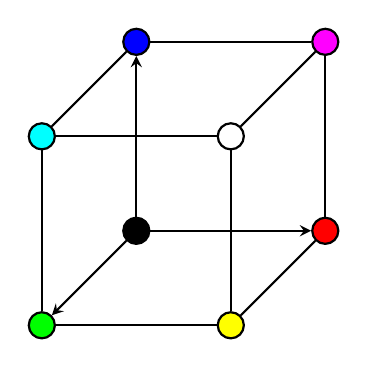
\begin{tikzpicture}
      \newcommand{\dist}[0]{24mm}
      \newcommand{\zdist}[0]{12mm}
      
      \tikzstyle{node}=[
        draw,
        circle,
        minimum height=0.2cm,
        minimum width=0.2cm,
        anchor=center,
        thick
      ]
      \tikzstyle{arrow} = [thick,->,>=stealth, draw=black]
      \tikzstyle{line} = [thick, draw=black]
      
      \definecolor{mycyan}{rgb}{0.0,1.0,1.0}
      \definecolor{mymagenta}{rgb}{1.0,0.0,1.0}
      \definecolor{myyellow}{rgb}{1.0,1.0,0.0}
      
      \node[node, fill=blue]      (blue)    at (0    , 0) {};
      \node[node, fill=mymagenta] (magenta) at (\dist, 0) {};
      \node[node, fill=black]     (black)   at (0    , -\dist) {};
      \node[node, fill=red]       (red)     at (\dist, -\dist) {};
      \node[node, fill=mycyan]   (cyan)   at (0-\zdist    , 0-\zdist) {};
      \node[node, fill=white]    (white)  at (\dist-\zdist, 0-\zdist) {};
      \node[node, fill=green]    (green)  at (0-\zdist    , -\dist-\zdist) {};
      \node[node, fill=myyellow] (yellow) at (\dist-\zdist, -\dist-\zdist) {};
      
      \draw[arrow] (black) -- (red);
      \draw[arrow] (black) -- (green);
      \draw[arrow] (black) -- (blue);
      \draw[line] (blue) -- (magenta);
      \draw[line] (blue) -- (cyan);
      \draw[line] (red) -- (magenta);
      \draw[line] (red) -- (yellow);
      \draw[line] (green) -- (yellow);
      \draw[line] (green) -- (cyan);
      \draw[line] (white) -- (cyan);
      \draw[line] (white) -- (magenta);
      \draw[line] (white) -- (yellow);
    \end{tikzpicture}
  }
\end{center}
